\documentclass[a4paper]{article}
\usepackage[utf8]{inputenc}
\usepackage[italian]{babel}
\usepackage[hidelinks]{hyperref}
\usepackage{graphicx}
\usepackage{pdfpages}
\usepackage{subfig}
\usepackage{float}
\usepackage{listings}
\usepackage{xcolor}
\usepackage[backend=biber,style=numeric-comp,maxbibnames=10]{biblatex}
\addbibresource{bibliography.bib}
\definecolor{codegreen}{rgb}{0,0.6,0}
\definecolor{backcolour}{rgb}{0.95,0.95,0.95}
\definecolor{codepurple}{rgb}{0.58,0,0.82}
\lstdefinestyle{style}{
    backgroundcolor=\color{backcolour},   
    commentstyle=\color{codegreen},
    keywordstyle=\color{magenta},
    stringstyle=\color{codepurple},
    basicstyle=\ttfamily\footnotesize,
    breakatwhitespace=false,         
    breaklines=true,                 
    captionpos=b,                    
    keepspaces=true,                 
    numbers=left,                    
    numbersep=5pt,                  
    showspaces=false,                
    showstringspaces=false,
    showtabs=false,                  
    tabsize=2
}
\lstset{style=style}
\title{
	Assignment 1 \\
	\large Visual Information Processing and Management}
\author{Davide Costantini, 856114}
\date{23 ottobre 2025}
\begin{document}
	\maketitle
	\newpage
	\section{Color Transfer}
	\begin{figure}[H]
		\centering
		\subfloat[][Mare torbido\cite{LitoraleFlegreo}]
		{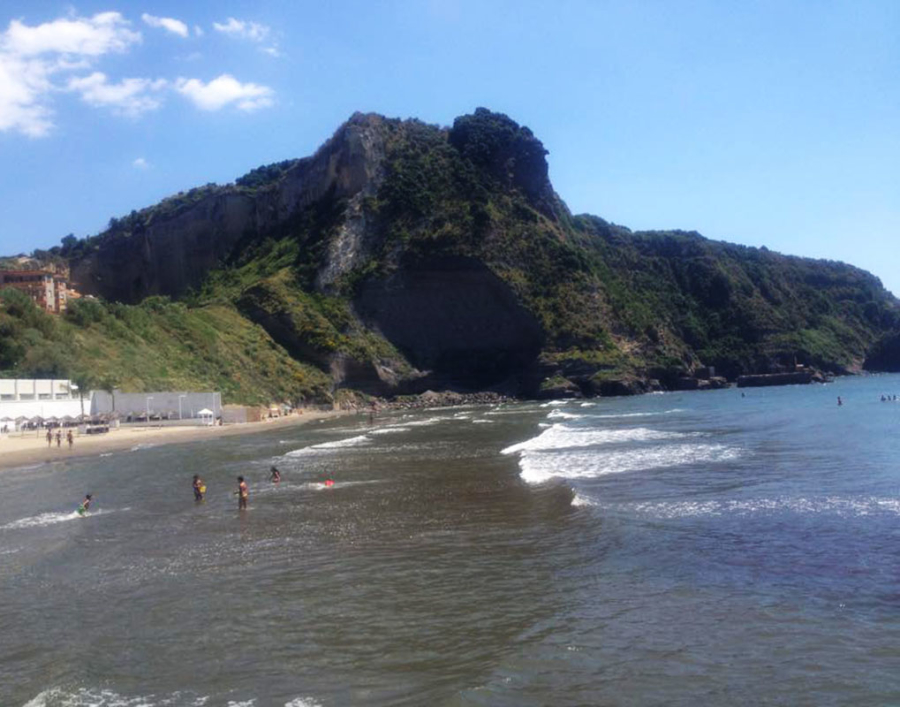
\includegraphics[width=0.49\columnwidth]{../colorTransfer/assignment/mare_torbido}}
		\hspace{0.05pt}
		\subfloat[][Mare limpido\cite{Calabria}]
		{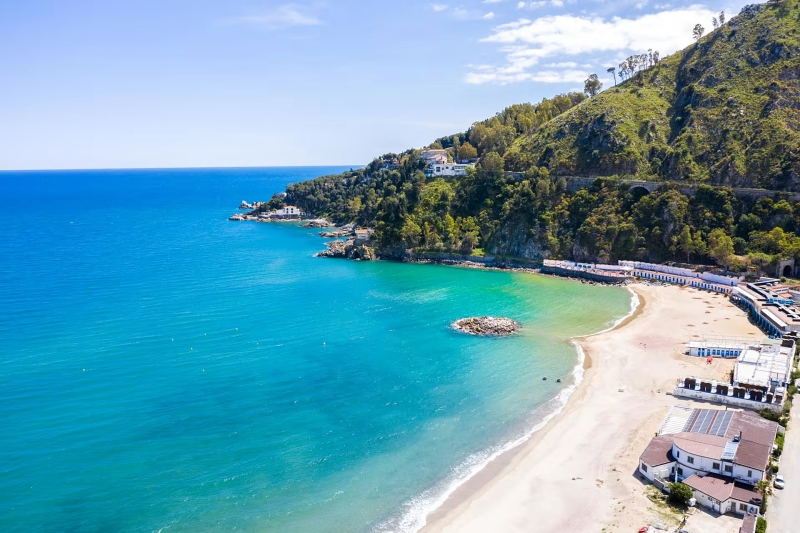
\includegraphics[width=0.49\columnwidth]{../colorTransfer/assignment/mare_limpido}}
		\caption{Immagini originali Color Transfer}
	\end{figure}
	\begin{figure}[H]
		\centering
		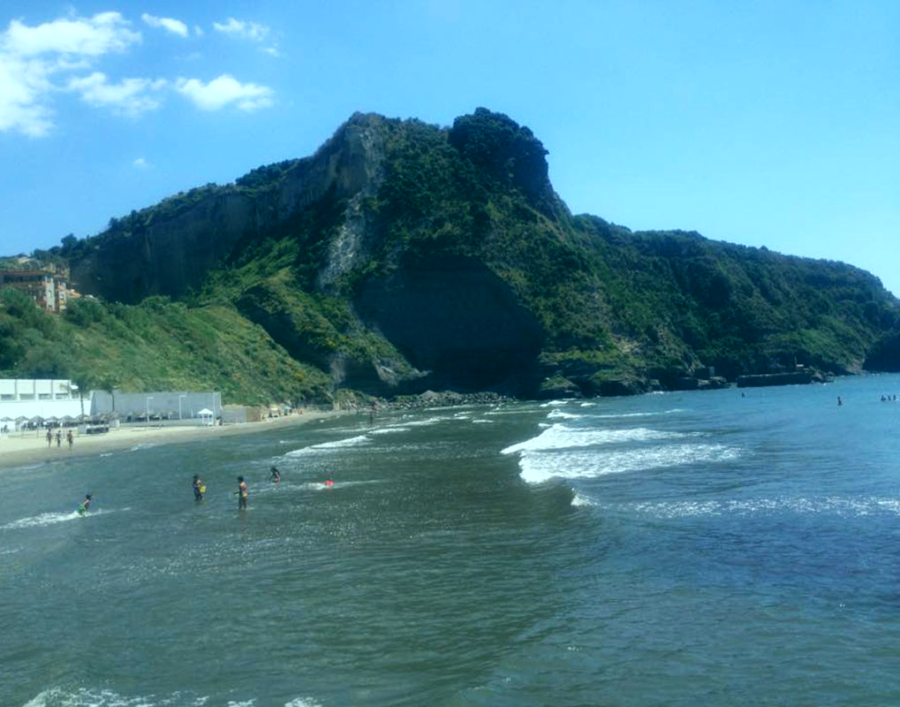
\includegraphics[width=\columnwidth]{images/color_transfer}
		\caption{Risultato}
	\end{figure}

	\newpage
	\section{Chroma Key}

	La parte di definizione del modello è stata modificata in modo da andare a prelevare più sezioni dell'immagine,
	tutte di dimensione 10x10 a partire dai pixel definiti nel vettore crops. La soglia è stata leggermente aumentata.  

	\begin{lstlisting}[language=Matlab, caption={Definizione del modello}]
	model = [];
	crops = [[140 40]; [560 410]; [470 490]];
	for ii = 1:size(crops, 1)
		crop = im1(crops(ii, 1):crops(ii, 1) + 10,
				   		 crops(ii, 2):crops(ii, 2) + 10, :);
		crop = reshape(crop, [], 3);
		crop = unique(crop, "rows");
		model{ii} = crop;
	end
	T = 0.13; \end{lstlisting}

	Di seguito sono illustrate le sezioni dell'immagine che sono state utilizzate per la definizione del modello.
	\begin{figure}[H]
		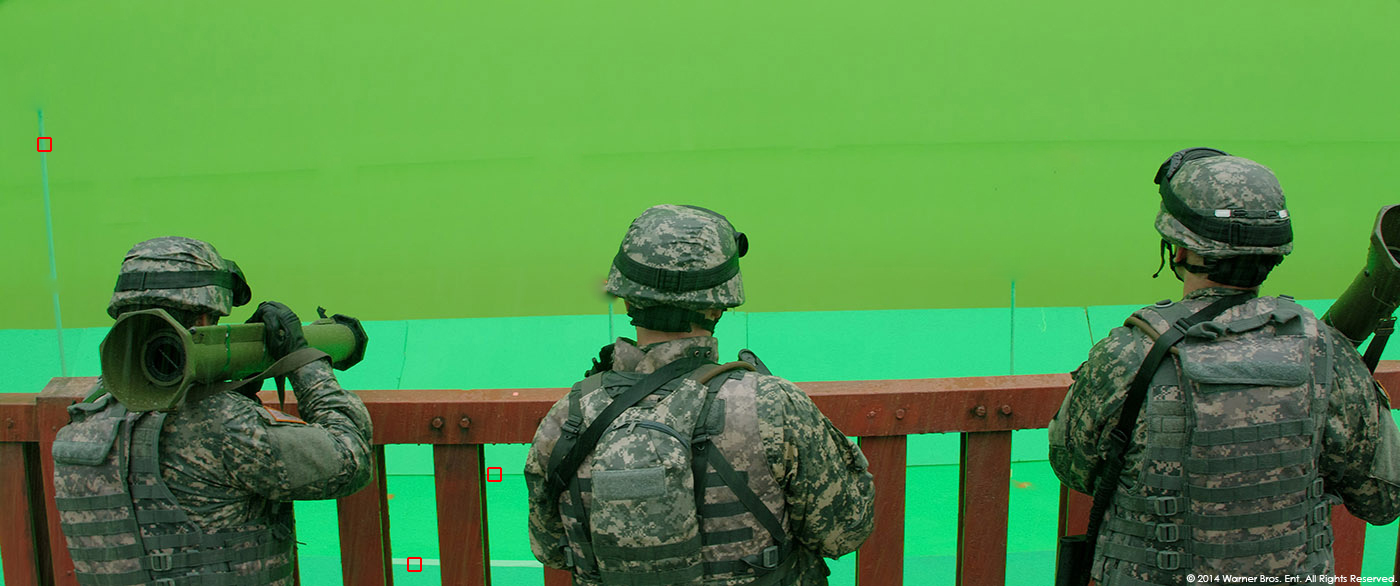
\includegraphics[width=\columnwidth]{images/crops_area}
		\caption{Crops utilizzati}
	\end{figure}

	La creazione della maschera è stata modificata in modo da crearne una per ogni crop ed unirle maschera finale
	effettuandone l'and logico.
	\begin{lstlisting}[language=Matlab, caption={Creazione della maschera}]
	M = ones(size(im1));
	for ii = 1:size(model, 2)
		tmp = zeros(size(im1));
		d = pdist2(im1, model{ii});
		tmp(min(d, [], 2) > T, :) = 1;
		M = M & tmp;
	end
	M = double(M); \end{lstlisting}

	\newpage

	L'immagine di seguito è il risultato dell'applicazione del chroma key utilizzando la maschera ottenuta.
	\begin{figure}[H]
		\centering
		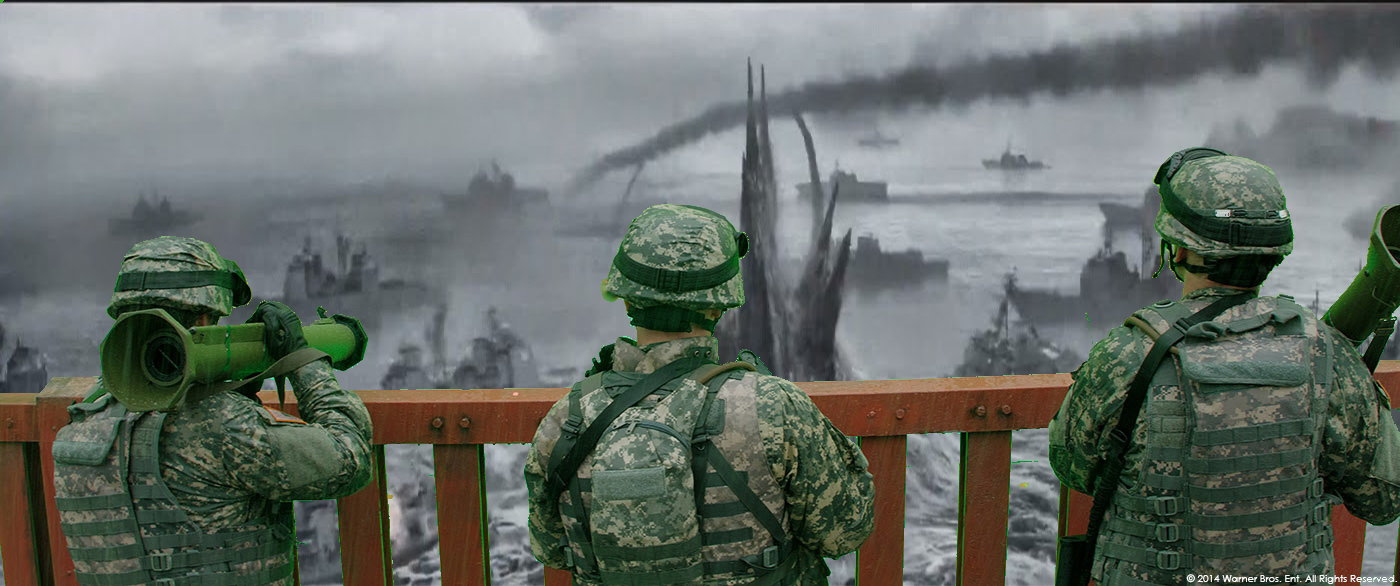
\includegraphics[width=\columnwidth]{images/chroma_key}
		\caption{Risultato}
	\end{figure}

	Infine, nella seguente immagine è riportato il risultato dell'applicazione del color transfer dall'immagine
	contenente lo sfondo all'immagine del chroma key.
	\begin{figure}[H]
		\centering
		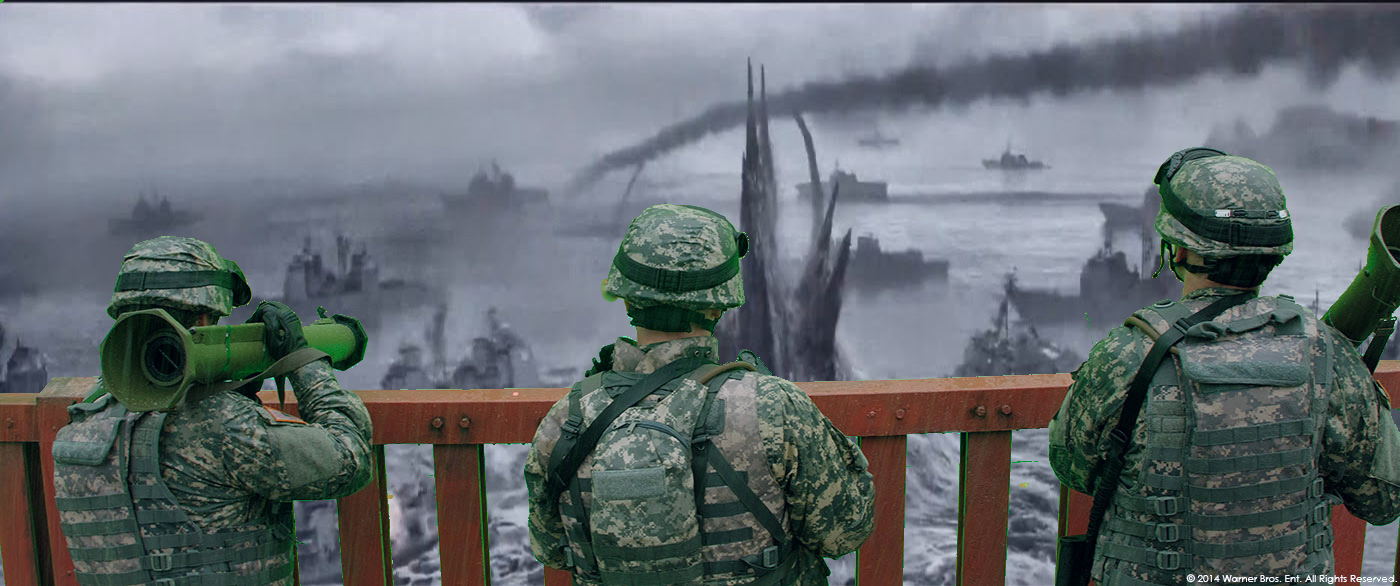
\includegraphics[width=\columnwidth]{images/chroma_key_and_color_transfer}
		\caption{Chroma key + color transfer}
	\end{figure}

	\newpage
	\printbibliography
\end{document}
